% The Saudi Legal Corpus for AI — resource paper.
%
% Venue-ready for the ACL style family (used by the NLLP workshop): drop the
% official acl.sty / acl_natbib.bst next to this file and it is used
% automatically. Without them, a self-contained two-column fallback layout
% compiles with a plain TeX Live so the draft can always be built and read.
% For LREC, swap the class/style per that year's official kit; the body needs
% no changes.
\documentclass[11pt]{article}

\IfFileExists{acl.sty}{%
  \usepackage[review]{acl}%
  \newcommand{\usingaclstyle}{}%
}{%
  % Fallback layout approximating ACL geometry.
  \usepackage[a4paper,top=2.5cm,bottom=2.5cm,left=2.5cm,right=2.5cm]{geometry}
  \usepackage{times}
  \usepackage[round]{natbib}
  \setlength{\columnsep}{0.6cm}
  \usepackage{multicol}
  % The ACL style loads hyperref itself; the fallback must provide it for \href.
  \usepackage[hidelinks]{hyperref}
}

\usepackage[T1]{fontenc}
\usepackage[utf8]{inputenc}
\usepackage{microtype}
\usepackage{booktabs}
\usepackage{graphicx}
\usepackage{url}

% Narrow two-column measure + many unhyphenatable \texttt identifiers:
% let TeX stretch interword space rather than overflow into the next column.
\emergencystretch=3em

\newcommand{\corpusname}{Saudi Legal Corpus for AI}

\title{The Saudi Legal Corpus for AI: An Auditable, Official-Source-Grounded,
Article-Level Corpus of Saudi Arabian Legislation}

\author{Abdullah Almohammedi \\
  Independent Researcher \\
  \texttt{abdullah.m.almohammedi@gmail.com} \\
  ORCID: \href{https://orcid.org/0009-0001-0832-0995}{0009-0001-0832-0995}}

\date{}

\begin{document}

\ifdefined\usingaclstyle
  \maketitle
\else
  \twocolumn[
    \maketitle
    \vspace{-2em}
  ]
\fi

\begin{abstract}
Legal NLP has advanced rapidly for English and European languages, but
Arabic --- and Saudi Arabian law in particular --- remains critically
under-resourced: to our knowledge, no openly documented, machine-readable,
article-level corpus of Saudi legislation has previously been described. We
present the \textbf{\corpusname}: 290 legislative instruments (201 statutory
laws, 64 statutory regulations, 24 implementing regulations, one set of
procedural rules) structured into \textbf{15{,}689 article-level records}
($\sim$1.2M Arabic tokens) in a unified, LLM-ready retrieval index. Three
design commitments distinguish it from web-scraped collections:
\emph{official-source grounding} (per-record provenance labels under a
four-tier source-verification taxonomy), \emph{auditability} (376
read-only, idempotent validators; fully deterministic derived layers), and
\emph{the governing-text principle} (the official Arabic text governs; all
other language layers are non-authoritative references). The corpus also
ships analytical layers that are, to our knowledge, the first of their kind
for Saudi law: a citation graph (3{,}607 references, 585 inter-law), a
hand-classified supersession graph (102 edges), a glossary of 1{,}920
statutorily defined terms, an embedding-ready chunking layer, and a
519-query manually confirmed retrieval benchmark. On it, the corpus's
metadata-based lexical searcher reaches 93.3\% top-1 accuracy versus 90.4\%
for a standard BM25 baseline, with the largest gap on definitional queries
(90.9\% vs.\ 74.5\%) --- quantifying the value of the engineered retrieval
metadata and leaving informative headroom for neural Arabic legal
retrieval. We describe the construction methodology, report reproducible
statistics, and discuss intended uses, limitations, and the legal and
ethical boundaries of releasing structured national legislation for AI
research.
\end{abstract}

\section{Introduction}

Large language models are increasingly consulted for legal questions, and
retrieval-augmented generation (RAG) over authoritative legal text is the
standard mitigation for hallucinated law. That mitigation, however, is only
available where authoritative legal text exists in machine-readable,
retrieval-ready form. For the law of the Kingdom of Saudi Arabia --- a G20
economy that has recently undergone a major codification wave, including a
new Civil Transactions Law (721 articles), a new Companies Law (281
articles), a new Evidence Law, and a new Personal Status Law --- no such
resource has, to our knowledge, been publicly documented. Saudi legislation is published
officially in the \emph{Umm Al-Qura} gazette and on government portals as
human-readable pages and PDFs; it is not distributed as structured,
article-level, provenance-annotated data.

This paper presents the \textbf{\corpusname}, which closes that gap. The
corpus structures the principal body of Saudi legislation into canonical
article-level JSON with explicit provenance, wraps it in deterministic
validation, and derives from it a unified retrieval index, a chunking layer,
citation and supersession graphs, a glossary of statutory definitions, and a
manually verified retrieval benchmark.

Our contributions are:

\begin{enumerate}
  \item \textbf{The corpus itself}: 291 legislative tracks, 15{,}689
    article-level records, $\sim$1.2M Arabic tokens, covering statutory law,
    regulations, implementing regulations, procedural rules, model
    contracts, and official annexes across commercial, civil, criminal,
    labor, financial, real-estate, technology, health, and administrative
    domains (Section~\ref{sec:contents}).
  \item \textbf{A methodology for auditable legal corpora}: official-source
    grounding with per-record provenance labels, a four-tier
    source-verification taxonomy, a freshness manifest that documents known
    staleness risks instead of hiding them, and 376 read-only idempotent
    validators (Section~\ref{sec:design}). We argue this methodology is a
    reusable template for legal corpora in any jurisdiction without a
    machine-readable official gazette.
  \item \textbf{Derived analytical layers} unavailable anywhere else for
    Saudi law: a cross-reference graph, a hand-classified supersession
    graph, and a statutory-definition glossary
    (Section~\ref{sec:layers}).
  \item \textbf{A retrieval evaluation resource}: 519 manually confirmed
    gold queries over the unified index, with two deterministic baselines
    --- the corpus's metadata-based lexical searcher (top-1 $=$ 93.3\%) and
    standard BM25 (top-1 $=$ 90.4\%) --- reported per query category so
    that future neural Arabic legal retrievers can be measured against both
    (Section~\ref{sec:retrieval}).
\end{enumerate}

Throughout, the corpus maintains a strict legal-status boundary: it is
\textbf{not} an official government publication, contains \textbf{no
official translation}, and the \textbf{official Arabic text governs};
English and Chinese layers are non-authoritative references. We return to
these boundaries in Section~\ref{sec:ethics}.

\section{Related Work}

\paragraph{Legal corpora and benchmarks.}
Large legal text collections and benchmarks now exist for English and
several European jurisdictions: the Pile of Law
\citep{henderson2022pileoflaw}, MultiLegalPile
\citep{niklaus2024multilegalpile}, LexGLUE \citep{chalkidis2022lexglue},
LEXTREME \citep{niklaus2023lextreme}, CUAD \citep{hendrycks2021cuad}, and
LegalBench \citep{guha2023legalbench}. These resources are dominated by
English and European languages; none includes Saudi legislation, and Arabic
is at most marginally represented.

\paragraph{Arabic legal NLP.}
Arabic NLP infrastructure has matured \citep[e.g.,][]{antoun2020arabert,
obeid2020camel}, and domain-specific models such as AraLegal-BERT
\citep{alqurishi2022aralegal} have been trained on proprietary Arabic legal
text. However, openly documented \emph{data resources} for Arabic law ---
in particular structured, provenance-annotated statute corpora --- remain
scarce. To our knowledge, no prior published resource provides
article-level, machine-readable coverage of Saudi legislation with
documented official-source provenance.

Table~\ref{tab:comparison} positions the \corpusname\ against these
resources. It is smaller by raw volume --- deliberately: it is a
\emph{structured statute corpus}, not a pretraining dump --- and it is the
only one that is article-level, Arabic-governing, and provenance-annotated
per record.

\begin{table*}[t]
\centering
\footnotesize
\begin{tabular}{lllll}
\toprule
\textbf{Resource} & \textbf{Type} & \textbf{Languages} & \textbf{Unit} & \textbf{Provenance} \\
\midrule
Pile of Law & pretraining corpus & English & document & no \\
MultiLegalPile & pretraining corpus & 24 (no Arabic) & document & per source \\
LexGLUE & benchmark & English & task example & no \\
LEXTREME & benchmark & 24 (no Arabic) & task example & no \\
LegalBench & benchmark & English & task example & no \\
\midrule
\corpusname & statute corpus $+$ eval & Arabic (gov.); EN/ZH ref. & article & per record \\
\bottomrule
\end{tabular}
\caption{Positioning against existing legal corpora and benchmarks. ``gov.''
= governing layer; ``ref.'' = non-authoritative reference layers (English
and Chinese currently cover one law). Per-record provenance here means 251
distinct source-status labels under a four-tier verification taxonomy.}
\label{tab:comparison}
\end{table*}

\paragraph{Legal document standards and citation networks.}
Standards such as Akoma Ntoso \citep{palmirani2011akoma} and the European
Legislation Identifier define structural markup for legislation; our
canonical JSON is deliberately simpler (flat article-level records with rich
retrieval metadata) but is convertible to such standards. A separate
literature applies network science to legal citation structure
\citep{fowler2007network, katz2014complexity, coupette2021measuring}; the
cross-reference and supersession graphs we release
(Section~\ref{sec:layers}) are, to our knowledge, the first
machine-readable inputs enabling that line of work for Saudi --- and more
broadly Gulf --- legislation.

\section{Source Material: The Saudi Legislative Landscape}
\label{sec:sources}

Saudi legislation is enacted primarily by royal decree
(\emph{ni\d{z}\={a}m} --- conventionally ``law'' or ``system'') and
elaborated by implementing regulations issued by ministers or authorities,
alongside procedural rules, ministerial decisions, and official model
forms. The authoritative publication channel is the official gazette
\emph{Umm Al-Qura}; consolidated texts are additionally published on
official portals, principally the Bureau of Experts at the Council of
Ministers (\url{laws.boe.gov.sa}) and the Ministry of Justice legal portal
(\url{laws.moj.gov.sa}), as well as issuing ministries' and authorities'
own sites.

\paragraph{Terminology.} Three unit terms recur in this paper and in the
data, at different granularities. A \textbf{track} is the registry's unit of
management: one onboarded instrument-layer bundle with its own sources,
validators, and reports (291 tracks, of which 290 correspond to legislative
instruments and one is a repository-level audit artifact). An
\textbf{instrument} (\texttt{law\_id}) is one enacted law, regulation, or
rule set as identified in the unified index (283 appear there). A
\textbf{corpus} (\texttt{corpus} key) is a subject-matter grouping that
typically joins a law with its implementing regulation and annexes --- e.g.,
the \texttt{labor} corpus spans eight components --- of which there are 199.

Each track records its Arabic and English display names, issuing authority,
official source URL(s), publication dates (Hijri and Gregorian where
available), language layers, record counts, and validator targets, in a
central machine-readable registry (registry version~3.0).

\section{Corpus Design and Methodology}
\label{sec:design}

\subsection{Design principles}

The corpus is built around four commitments:

\begin{enumerate}
  \item \textbf{Official Arabic text governs.} Every record carries the
    official Arabic text verbatim (\texttt{text\_ar}); no summarization,
    normalization, or editorial rewriting is applied to the governing text.
    All non-Arabic layers are explicitly flagged as non-authoritative.
  \item \textbf{Provenance is per-record and honest.} Every record in the
    unified index carries a \texttt{text\_status} provenance label
    describing exactly how its text was obtained and verified (e.g.,
    cross-checks between the Ministry of Justice portal API and published
    official PDFs). There are 251 distinct provenance labels ---
    deliberately fine-grained rather than collapsed, because collapsing
    provenance destroys auditability. Where the primary portal was found
    stale at build time (e.g., an unincorporated amendment), that is
    documented, not silently patched: the freshness manifest flags 16 of
    291 tracks with a known source-staleness risk.
  \item \textbf{Validation is read-only, deterministic, and idempotent.}
    The repository ships 376 validator targets (of 476 total build targets)
    that check schema conformance, record counts, hashes, layer boundaries,
    and cross-layer consistency without mutating any data. Derived-layer
    generators make no network calls and use no wall-clock time, so every
    layer is exactly reproducible from the committed sources.
  \item \textbf{Derived layers are additive projections.} The unified
    index, chunking layer, graphs, glossary, tiers, and freshness manifest
    are all read-only projections over the canonical track files. None of
    them alters legal text; each records what it was generated from.
\end{enumerate}

\subsection{Source verification tiers}

Because Saudi Arabia has no machine-readable official gazette, source
quality varies by track and must be represented rather than assumed. Every
track is assigned to one of four verification tiers
(Table~\ref{tab:tiers}). This taxonomy lets downstream users filter by
evidential strength --- a RAG deployment may restrict itself to
Tiers~1--2, while a coverage-oriented study may accept all four with the
caveats attached.

\begin{table}[t]
\centering
\small
\begin{tabular}{p{5.2cm}r}
\toprule
\textbf{Tier} & \textbf{Tracks} \\
\midrule
1 --- primary, multi-source & 127 \\
2 --- primary $+$ secondary cross-verified & 88 \\
3 --- secondary multi-source only & 39 \\
4 --- single-source or mixed confidence & 37 \\
\bottomrule
\end{tabular}
\caption{Source-verification tier assignments (291 tracks).}
\label{tab:tiers}
\end{table}

\subsection{Record schema}

The atomic unit is the \textbf{article-level record}
(Figure~\ref{fig:record}). In the unified retrieval index each record
carries: a stable \texttt{record\_id}; corpus/track identifiers
(\texttt{corpus}, \texttt{law\_id}, \texttt{law\_component}); the official
Arabic law title and article number; generated retrieval metadata
(\texttt{llm\_title\_ar}, \texttt{retrieval\_title\_ar},
\texttt{keywords\_ar}, \texttt{search\_queries\_ar}); the verbatim
governing text (\texttt{text\_ar}); the provenance label
(\texttt{text\_status}); and the source layer file it was projected from.
Records are self-contained: a single retrieved record is sufficient context
to cite the law, component, and article.

\begin{figure*}[t]
\centering
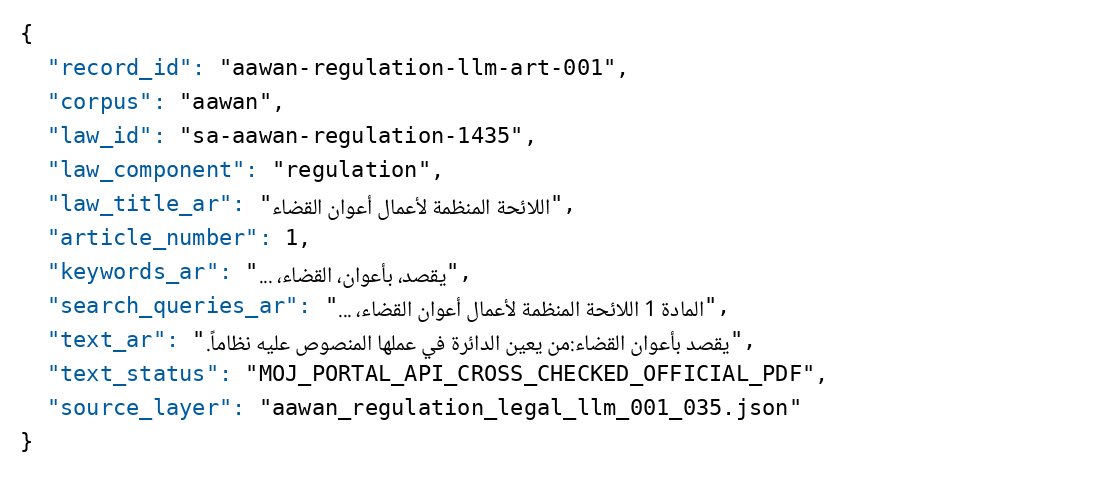
\includegraphics[width=0.92\textwidth]{example_record.png}
\caption{An example unified-index record (Article~1 of the Regulation of
Judicial Assistants' Work, abridged: keyword and query lists truncated).
The article text translates as: ``Judicial assistants means: those who
assist the circuit in its work as prescribed by law.'' The
\texttt{text\_status} label records that the text was cross-checked between
the Ministry of Justice portal API and the published official PDF.}
\label{fig:record}
\end{figure*}

\subsection{Metadata generation and AI-usage disclosure}
\label{sec:disclosure}

Resource papers increasingly document not only what a dataset contains but
how each field came to be \citep{bender2018data, gebru2021datasheets}. In
this corpus: (i)~the governing Arabic text (\texttt{text\_ar}) is ingested
verbatim from the recorded official sources and is never generated,
summarized, or normalized; validators enforce this by hash and count.
(ii)~The retrieval metadata is produced \emph{mechanically} by each track's
deterministic generator script --- keywords by term-frequency extraction
from the article's own text, search queries and retrieval titles by
number/title templates --- not by a generative model, which is why the
metadata-based searcher of Section~\ref{sec:retrieval} is deterministic
end-to-end. (iii)~The non-governing reference layers (English, and the
internal Chinese layer) were produced with machine-assisted translation and
passed a documented internal QA program; they are explicitly non-official
and non-binding. (iv)~Repository tooling and documentation were developed
with AI assistance; every data-bearing layer that tooling produces is
regenerable deterministically and checked by read-only validators.

\section{Corpus Contents and Statistics}
\label{sec:contents}

All figures are computed by the accompanying read-only script and stored
alongside the corpus.

\subsection{Track-level composition}

\begin{table}[t]
\centering
\small
\begin{tabular}{lr}
\toprule
\textbf{Corpus family} & \textbf{Tracks} \\
\midrule
Statutory laws & 201 \\
Statutory regulations & 64 \\
Implementing regulations & 24 \\
Procedural rules & 1 \\
Closure-audit track & 1 \\
\midrule
\textbf{Total} & \textbf{291} \\
\bottomrule
\end{tabular}
\caption{Track-level composition of the corpus.}
\label{tab:families}
\end{table}

Track composition is shown in Table~\ref{tab:families}; the closure-audit
track is a repository-level QA artifact, not legislation, and carries no
legal text. The registry counts 16{,}753 records in total: 15{,}858 primary
Arabic governing records, 614 reference records (English layers), and 281
internal reference records (the Chinese internal layer for the Companies
Law). The unified retrieval index (next subsection) projects 15{,}689 of
the primary governing records; the remaining 169 belong to the separate
implementing-regulations intake track family, which is registry-counted but
served through its own layer files. Its 15{,}689 records span 283 distinct
instruments grouped into 199 subject-matter corpora (per the terminology of
Section~\ref{sec:sources}).

\subsection{The unified retrieval index}

The unified LLM retrieval index projects the retrieval-relevant records
into one file; Table~\ref{tab:index} summarizes it and
Table~\ref{tab:components} breaks records down by component type.

\begin{table}[t]
\centering
\small
\begin{tabular}{lr}
\toprule
\textbf{Measure} & \textbf{Value} \\
\midrule
Article-level records & 15{,}689 \\
Distinct legislative instruments & 283 \\
Distinct corpora & 199 \\
Arabic tokens (whitespace) & 1{,}206{,}097 \\
Characters & 7{,}123{,}487 \\
Distinct provenance labels & 251 \\
\bottomrule
\end{tabular}
\caption{The unified retrieval index at a glance.}
\label{tab:index}
\end{table}

\begin{table}[t]
\centering
\small
\begin{tabular}{lr}
\toprule
\textbf{Component} & \textbf{Records} \\
\midrule
Law articles & 8{,}384 \\
Regulation articles & 4{,}655 \\
Implementing-regulation articles & 2{,}113 \\
Procedural manuals & 135 \\
Model contract forms & 102 \\
Model work regulation & 75 \\
Recruitment services rules & 72 \\
Other rules, guides, annexes & 153 \\
\bottomrule
\end{tabular}
\caption{Unified-index records by component type.}
\label{tab:components}
\end{table}

Coverage spans the core commercial stack (Companies Law, Bankruptcy,
Commercial Courts, Capital Market, Banking Control), the new codification
wave (Civil Transactions --- 721 articles, Evidence, Personal Status),
criminal and procedural law (Criminal Procedure, Sharia Procedure and its
637-article regulation, Enforcement), labor and social insurance (including
official annexes: violation tables, model contracts), technology and data
(the Personal Data Protection Law and its regulations, E-Commerce,
Electronic Transactions, Cybersecurity), tax and zakat (VAT, RETT, Income
Tax, Zakat), real estate (registration, brokerage, finance, off-plan sales,
contributions), health, environment, media, transport, and the
institutional statutes of major authorities.

\subsection{Multilingual layers}

The Saudi Companies Law (Royal Decree M/132, 1443H; 281 articles) is the
first track with full multilingual treatment: the governing Arabic layer, a
full English LLM layer (281 records), an English reference layer (281
records), and an internal Chinese reference layer that passed a documented
four-phase remediation and QA program, closed by a repository-level audit.
The corpus explicitly does \textbf{not} claim trilingual alignment or an
official translation; the multilingual layers exist to support
cross-lingual access research under the governing-text principle.

\section{Derived Analytical Layers}
\label{sec:layers}

\subsection{Cross-reference graph}

A deterministic extractor scans all 15{,}689 records for statutory
citations, yielding \textbf{3{,}607 references}: 3{,}022 intra-law and
\textbf{585 inter-law} citations, emitted with the raw citation text,
source/target identifiers, and a confidence label (3{,}087 high, 520
medium; 0 ambiguous-scope). The 585 inter-law edges span 191 distinct
source tracks and 316 distinct cited target names; the most-cited targets
are the Labor Law (34 inbound citations), the Companies Law (30), the
Bankruptcy Law (19), and the Sharia Procedure Law (14). This is, to our
knowledge, the first machine-readable citation network over Saudi
legislation, and it directly enables network-science studies of the Saudi
legal system (centrality, clustering, dangling references to superseded
instruments).

\subsection{Supersession graph}

A separate layer records repeal/replacement relationships between
instruments: \textbf{102 edges}, each classified \emph{by hand} against the
corpus's own documented text (registry notes and official-source metadata)
--- never inferred from decree age or topical similarity. Ambiguous cases
and title-collision non-repeals are kept in their own sections rather than
forced into edges. Combined with the citation graph, this supports temporal
legal dynamics research (e.g., which live laws still cite repealed ones).

\subsection{Statutory-definition glossary}

Saudi laws conventionally open with a definitions article. A parser over
these articles yields a corpus-wide glossary of \textbf{1{,}920 terms} with
\textbf{3{,}318 definitions}, extracted from the 214 tracks whose
definitions articles parse cleanly. Because the same term (e.g.,
``establishment'', ``competent authority'') is defined independently by
many laws, the glossary is the raw material for studying definitional
fragmentation and terminological consistency across a national legal
system.

\subsection{Freshness manifest}

A deterministic, network-free manifest surveys every track's recorded
source URLs, fetch dates, and known discrepancies, and flags \textbf{16
tracks} with a documented risk that the primary portal's consolidated text
was stale at build time. A separate live checker (explicitly outside the QA
gate) can re-probe reachability and drift.

\section{Retrieval Index, Chunking, and Baseline Evaluation}
\label{sec:retrieval}

\subsection{Chunking layer}

For embedding pipelines, a chunking layer segments the unified index into
\textbf{16{,}304 chunks} sized in whitespace words (deliberately not tied
to any specific embedding tokenizer). 15{,}344 records fit in a single
chunk; 345 long articles are split, with each chunk carrying its source
record identifier, article number, chunk index, and exact character offsets
into the source text, so any vector hit is traceable to its governing
article. No embeddings are computed in-repository; the layer is pure,
traceable segmentation.

\subsection{Gold-query evaluation set}

The retrieval evaluation pack contains \textbf{519 Arabic queries}, each
with a manually confirmed gold article (corpus, component, article number).
Golds were confirmed against the articles' own text or official structure
--- not reverse-engineered from search output --- so the metrics honestly
measure the searcher. Queries are categorized: 384 topical, 61
provision-lookup, 55 definitional, and 19 in smaller categories
(governance, rights, procedural, and deliberately hard cases).

\paragraph{Annotation disclosure.} The queries and golds were authored by a
single annotator (the corpus maintainer), by reading each article's
committed text first and writing the query from its own wording; there is
consequently no inter-annotator agreement to report, and the set inherits
an in-vocabulary bias that we quantify next. Provision-lookup queries
(``Article~5 of the Labor Law'') share their surface form with the
templated \texttt{search\_queries\_ar} metadata, so for that category the
evaluation partly measures template matching rather than free-form
retrieval --- the per-category breakdown below keeps this visible instead
of averaging it away.

\subsection{Baseline results}

We report two deterministic baselines. The \textbf{metadata searcher} is the
corpus's own lexical scorer over each record's generated retrieval metadata
(weighted keyword/title/query matching; no embeddings, no learned
parameters). \textbf{BM25} is standard Okapi BM25 ($k_1{=}1.5$, $b{=}0.75$)
over each record's law title, article title, and verbatim text, with light
Arabic orthographic normalization (diacritics and tatweel stripped; alef,
teh-marbuta, and alef-maqsura variants folded) and whitespace tokenization
--- no stemming, no stopword list. Table~\ref{tab:baseline} reports overall
and per-category results (the 19 small-category queries are included in the
overall row but not broken out).

\begin{table}[t]
\centering
\small
\begin{tabular}{lrrrr}
\toprule
 & \multicolumn{2}{c}{\textbf{Metadata}} & \multicolumn{2}{c}{\textbf{BM25}} \\
\textbf{Queries} & \textbf{T@1} & \textbf{MRR} & \textbf{T@1} & \textbf{MRR} \\
\midrule
All (519) & 93.3 & .956 & 90.4 & .937 \\
Topical (384) & 93.2 & .957 & 92.7 & .956 \\
Provision (61) & 98.4 & .984 & 98.4 & .984 \\
Definitional (55) & 90.9 & .937 & 74.5 & .809 \\
\bottomrule
\end{tabular}
\caption{Top-1 accuracy (\%) and MRR@5 on the 519-query evaluation set:
the corpus's metadata-based searcher vs.\ standard BM25 over titles $+$
verbatim text.}
\label{tab:baseline}
\end{table}

Three observations. First, the near-identical provision-lookup scores
confirm the template-matching effect disclosed above: both systems resolve
``Article $n$ of law $X$'' queries almost perfectly, so that category says
little about retrieval quality. Second, the gap concentrates exactly where
retrieval is hardest: on definitional queries --- where a query like
``definition of the sale contract'' shares few surface tokens with the
defining article --- the engineered metadata is worth $+16.4$ points of
top-1 accuracy over BM25 (90.9\% vs.\ 74.5\%). Third, six metadata-searcher
queries miss the top-5 entirely; per-query results for both systems are
published, making error analysis reproducible. The remaining headroom ---
and, more importantly, robustness to paraphrase and dialectal variation not
present in the gold queries --- is exactly the space in which neural Arabic
legal retrievers should be evaluated. We release the queries, golds,
per-query results, and both runner scripts to support that comparison.

\section{Intended Uses}
\label{sec:uses}

\begin{itemize}
  \item \textbf{RAG grounding for Saudi-law assistants}, with per-record
    provenance and verification tiers enabling deployments to filter by
    evidential strength.
  \item \textbf{Arabic legal-NLP research}: retrieval, summarization,
    question answering, terminology extraction, and cross-lingual legal
    access, over a morphologically rich, formulaic register of Modern
    Standard Arabic.
  \item \textbf{Computational legal studies}: citation-network analysis,
    definitional consistency, law-vs-regulation delegation studies,
    temporal dynamics of the 2022--2023 codification wave.
  \item \textbf{Benchmarking factuality}: the corpus provides ground truth
    for measuring LLM hallucination on Saudi legal questions.
  \item \textbf{A methodological template} for building auditable legal
    corpora in jurisdictions without machine-readable official gazettes.
\end{itemize}

\section{Limitations}
\label{sec:limitations}

\begin{itemize}
  \item \textbf{Not exhaustive.} 291 tracks cover the principal
    legislation, but not every ministerial decision, circular, or municipal
    instrument; coverage is documented per-track rather than claimed
    complete.
  \item \textbf{Consolidation risk.} Official portals themselves sometimes
    lag amendments; 16 tracks carry a documented staleness-risk flag, and
    37 tracks sit in the lowest verification tier. The corpus documents
    these risks; it cannot eliminate them.
  \item \textbf{Extraction layers are heuristic.} The cross-reference
    extractor and glossary parser are deterministic but pattern-based;
    their published caveats (confidence labels, skipped tracks) bound but
    do not remove extraction error. The supersession graph is
    hand-classified and therefore conservative and possibly incomplete.
  \item \textbf{The evaluation set is single-annotator and lexically close
    to the corpus.} The 519 gold queries were authored by one annotator
    from the articles' own wording (no inter-annotator agreement), and the
    provision-lookup category overlaps the templated query metadata
    (Section~\ref{sec:retrieval}); the set measures in-vocabulary retrieval
    well, paraphrase robustness less so.
  \item \textbf{Multilingual depth is uneven.} Only the Companies Law has
    full English and internal Chinese layers; the corpus is Arabic-first by
    design.
\end{itemize}

\section{Ethical and Legal Considerations}
\label{sec:ethics}

The corpus contains enacted national legislation --- public legal facts,
not personal data. Nevertheless, three boundaries are enforced
repository-wide and repeated here: the corpus is \textbf{not an official
government publication}; its non-Arabic layers are \textbf{not official
translations}; and nothing in it is \textbf{legal advice} --- the only
binding text is the Arabic original as published in \emph{Umm Al-Qura}. The
structuring apparatus (schemas, scripts, derived layers, metadata) is
released under the MIT license; the underlying statutory texts remain
public legal enactments of the Kingdom of Saudi Arabia, and the corpus
asserts no ownership over them. Field-level generation provenance is
documented in Section~\ref{sec:disclosure}, in the spirit of data
statements and datasheets \citep{bender2018data, gebru2021datasheets}. A
misuse consideration specific to legal corpora is over-trust: shipping
provenance labels, verification tiers, and staleness flags \emph{inside}
the data --- rather than in documentation users never read --- is a
deliberate design choice so that downstream systems can surface uncertainty
instead of laundering it.

\section{Conclusion and Future Work}

We presented the \corpusname: 290 legislative instruments and 15{,}689
article-level records of Saudi legislation with per-record provenance,
tiered source verification, deterministic validation, derived
citation/supersession/glossary layers, and a manually confirmed 519-query
retrieval benchmark with two deterministic baselines that already localize
where retrieval is hard (definitional queries). Future work proceeds on
three axes: (1)~neural baselines --- Arabic and multilingual embedding
models evaluated on the released benchmark, including paraphrase-robustness
extensions of the query set; (2)~analytical studies over the released
graphs --- legislative network structure, definitional fragmentation, and
the temporal dynamics of the Saudi codification wave; and (3)~coverage
growth --- onboarding further instruments through the same profile-driven
factory, with amendment-tracking as the hardest open problem for any legal
corpus in a jurisdiction without a machine-readable gazette.

\section*{Data Availability}

The corpus, all derived layers, all validators, the evaluation pack, and
the scripts reproducing every figure in this paper (corpus statistics, the
BM25 baseline, and the example-record figure) are available in the
repository \texttt{al3obdi/saudi-legal-corpus-ai}. \emph{[TODO before
submission: mint a versioned, DOI-carrying archival release (e.g., Zenodo)
and cite it here.]}

\IfFileExists{acl_natbib.bst}{%
  \bibliographystyle{acl_natbib}%
}{%
  \bibliographystyle{plainnat}%
}
\bibliography{references}

\end{document}
